\section{Theory}
\label{sec:theory}

\subsection{Photoluminescence}

To probe the band gap of semiconductors, photoluminescence spectroscopy can be used.
This means illuminating the sample in order to create electron-hole pairs, which then form excitons and ultimately recombine, sending out a photon.
The energy of the exciton annihilation is characteristic for the material.
Therefore a spectrum recorded by the emission of such an illuminated sample will contain a peak at this characteristic energy (wavelength) of the most favorable transition as well as possibly other peaks stemming from effects such as spin-splitting and phonon-activated transitions.

\subsection{Transition metal dichalcogenides}

TMDCs are layered materials made from one part transition metal (Mo, Ti, W) and two parts chalcogenides (S, Se, Te) and are typically semiconductors.
The general crystal structure is shown in \cref{fig_tmdc_structure}.
The layers can be separated from each other by exfoliation as they are only bound by comparatively weak Van der Waals bonds, while within the plane the atoms are bound by covalent bonds.
As monolayers, unlike the bulk crystal, don't have an inversion center, the band structure changes considerably, when transitioning from the bulk to monolayers.
Specifically the $\bar{K}$ points of the reciprocal lattice no longer show sixfold symmetry, and split into $\bar{K}$ and $\bar{K}'$ valleys, which have reversed splin splitting.
As shown in \cref{fig_valley_split}, this leads to the existence of lower energy A excitons and higher energy B excitons, which couple to different circular polarizations of light depending on the valley.

\begin{figure}[!ht]
    \centering
    \begin{subfigure}{0.47\textwidth}
        \centering
    		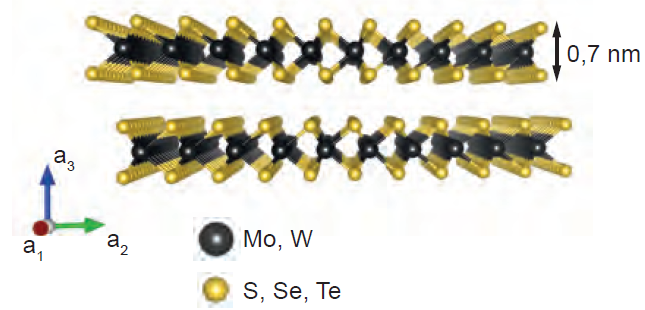
\includegraphics[width=\textwidth]{img/tmdc_structure.png}
    		\caption{}
    		\label{fig_tmdc_structure}
    \end{subfigure}
    \hfill
    \begin{subfigure}{0.37\textwidth}
        \centering
        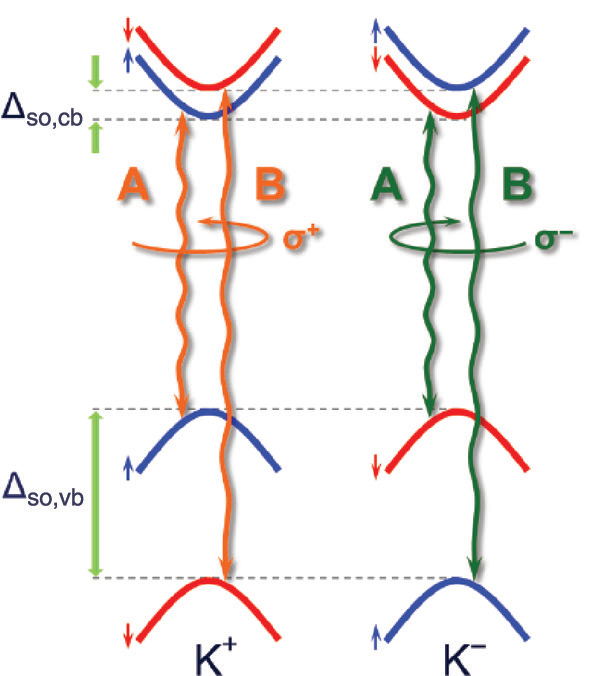
\includegraphics[width=\textwidth]{img/AB_exc.png}
        \caption{}
	      \label{fig_valley_split}
    \end{subfigure}
    \caption{a: Layered crystal structure of TMDCs. \cite{Schmidt2016}. b: Valley dependence on spin splitting in monolayer TMDCs.\cite{Koperski2017} }
	\label{fig_tmdcs} % 3->1
\end{figure}


\subsection{Single-photon emitters}
\label{sec:theory:spe}

Single-photon emitters (SPEs) are light sources that don't emit more than one photon at once.
SPEs are identified by performing photon antibunching, meaning that two detectors are used, whith one giving a start signal and the other the stop signal, allowing the measurement of the so called second-order correlation function
\begin{equation}
  g^{(2)}(\tau) = \frac{\left< I(t) I(t + \tau) \right>}{\left< I(t)\right> ^2} \,.
\end{equation}
Here $I(t)$ is the intensity trace and $\left< \right>$ refers to the expected value.
This function can be measured using the Hanbury-Brown-Twiss (HBT) inferometry setup depicted in \cref{fig_hbt}.
If the emitter in question is a Single-photon emitter, there will be a significant dip in the relative quantity of delays between start and stop signal close to zero \cite{tran2016}.
SPEs are defined as having this dip be below \SI{0.5}{} at $\tau = 0$, if the measurement is normalized to \SI{1}{} far away from the dip.

\begin{figure}[!ht]
    \centering
    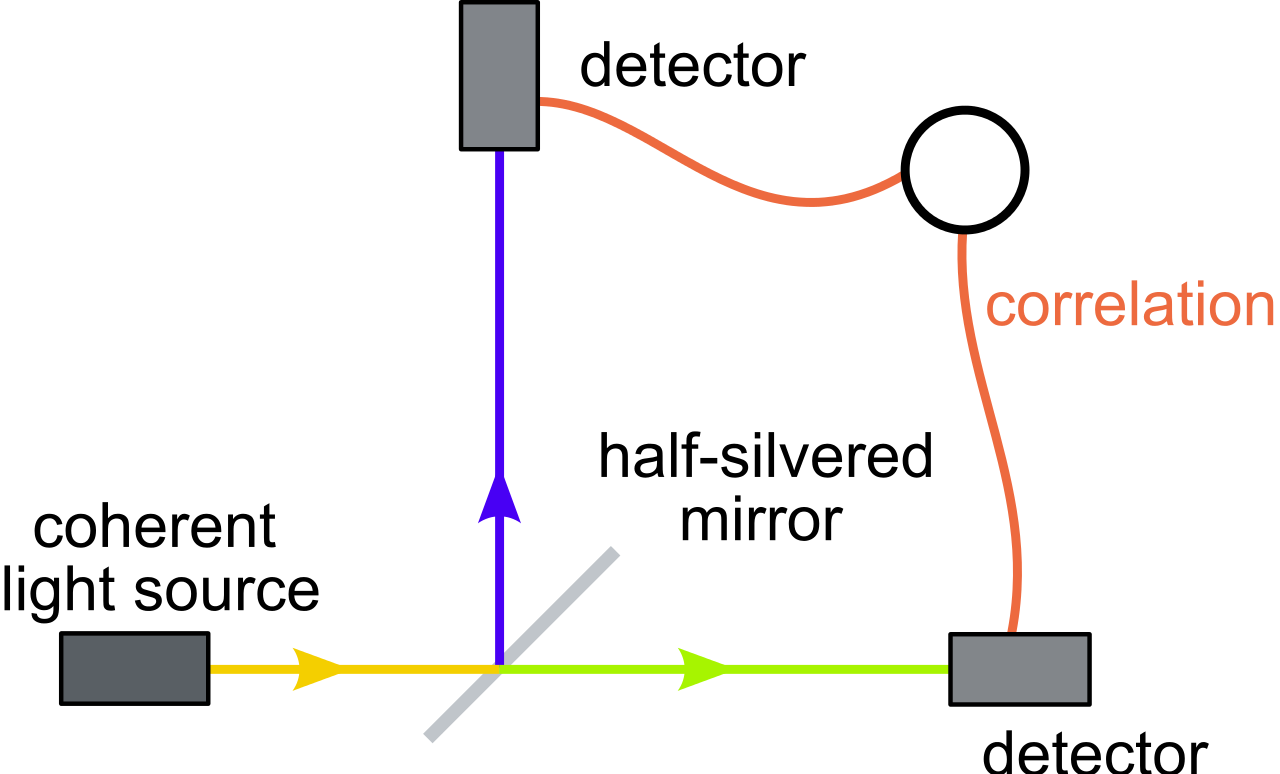
\includegraphics[width=0.6\textwidth]{img/Correlation-interferometer}
    \caption{Schematic of the Hanbury-Brown-Twiss experiment. \cite{wikiHBT}}
    \label{fig_hbt}
\end{figure}

\subsection{Magneto-optic effect}

	The interaction of electromagnetic waves with matter can be described with the refractive index
	\begin{align*}
		\tilde{n} = n + ik \,,
	\end{align*}
	where $n$ describes the refraction and $k$ the absorption.
	From this information on reflection and transmission can also be extracted.
	Adding an external magnetic field to the matter, changes its refractive index for different polarizations of the incoming electromagnetic wave.

  Linear polarized light can be described by a superposition of two circular polarized electromagnetic waves, one left- and one right-polarized.
	When passing through the matter, the left- and right-polarized parts change differently in intensity and phase.
	The result is that the superposition of both waves no longer adds to linear polarized, but elliptic polarized light.
	From the phase change results a rotation of the lights main oscillation axis and from the intensity change the ellipticity.
	This rotation is also known as Faraday rotation.
	Here, it should be noted that this is the case for transmission through matter.
  For reflection on the other hand a similiar effect, namely the magneto-optical Kerr effect, takes place.

	\

	As the change in polarization through interaction with magnetized matter is heavily dependent on the properties of the matter, band structure information can be obtained using magneto-optic methods.
	An example of this is given by spin polarized band gaps.
	For this investigation, the Zeeman-splitting for 1s-excitons in TMDCs and how they influence the refractive properties of matter is of interest.
	This can be described by the Verdet constant $V$ which is given by:
	\begin{align*}
		V = \frac{\varphi_\text{F}}{L\cdot B} \,,
	\end{align*}
	where $\varphi_\text{F}$ is the Faraday rotation, $L$ the thickness of the sample and $B$ the strength of the external magnetic field.

	To allow the deduction of the Faraday rotation by measurement of transmission intensities, Jones matrices can be used.
	They describe the change of polarization in the plane transverse to the light's direction of propagation.
	For example the sample can be described by
	\begin{align*}
		\hat{\text{S}} = \left( \begin{array}{rr}
		1 & (\varphi_\text{F} + i\eta_\text{F}) \\
		-(\varphi_\text{F} + i\eta_\text{F}) & 1 \\
	\end{array}\right) \,,
	\end{align*}
  with $\eta_\text{F}$ being the ellipticity of the polarization.
	The electric field of initially linearly polarized light $\hat{E}_i$ can be written as a two-component vector:
	\begin{align*}
		\hat{E}_i = \left( \begin{array}{r}
					\cos{p} \\
					\sin{p} \\
				\end{array}\right) \,,
	\end{align*}
	where $p$ describes the angle of the linear polarization.
	By multiplying this vector with the Jones matrices $\hat{J}_k$ of the different objects in the beams path, expressions for the measured intensities $T_i = E_i^* E_i$ can be calculated.
  Specifically, $E_i \propto \prod_k \hat{J}_k \cdot \hat{E}_i$.
  Here, the indices $i$ are assigned to the two components of the initially linear polarized light.

  The faraday rotation results from taking the difference of the measured intensities $T_i$ each divided by the intensities measured without a sample $T_i^0$:
	\begin{align*}
		\frac{T_1}{T_1^0} - \frac{T_2}{T_2^0} = 4 \varphi_\text{F} + \varphi_\text{bg} \,.
	\end{align*}
	Additionally, there is $\varphi_\text{bg}$, which amounts to noise expected to be measured without the sample.
